%==============================================================================
%  Speaker-Conditioned Verification and Lexicographic Tie-Breaking for
%  Hallucination Detection in Legislative Hearings
%  1o Desafio de Dados do Instituto Kunumi - 2026  (Ideias em Rede, 1a Edicao)
%
%  Compile:  pdflatex -> bibtex -> pdflatex -> pdflatex
%==============================================================================

\AddToHook{package/amssymb/before}{\let\Bbbk\undefined}
\documentclass[english]{desafiokunumi}
\graphicspath{{figures/}}

\usepackage{tikz}
\usepackage{needspace}
\usetikzlibrary{positioning,patterns,arrows.meta}
% amsthm colide com o \openbox do newtxmath carregado pela classe; liberamos o
% nome ANTES do load (o unico conflito restante, \Bbbk, e interno a classe)
\let\openbox\undefined
\usepackage{amsthm}

% O .cls fixa os rotulos "Resumo."/"Palavras-chave:" mesmo sob a opcao [english].
% Corrigimos aqui, a partir do main.tex, sem alterar o arquivo distribuido.
\usepackage{etoolbox}
\makeatletter
\patchcmd{\maketitle}{Resumo.}{Abstract.}{}{\typeout{[aviso] rotulo Resumo nao encontrado}}
\patchcmd{\maketitle}{Palavras-chave:}{Keywords:}{}{\typeout{[aviso] rotulo Palavras-chave nao encontrado}}
\makeatother

\newtheorem{theorem}{Theorem}
\newtheorem{proposition}[theorem]{Proposition}
\newtheorem{observation}[theorem]{Observation}
\newtheorem{corollary}[theorem]{Corollary}
\newtheorem{lemma}[theorem]{Lemma}
\theoremstyle{definition}
\newtheorem{definition}[theorem]{Definition}
\newtheorem{example}[theorem]{Example}
\theoremstyle{remark}
\newtheorem{remark}[theorem]{Remark}

\newcommand{\SE}{\mathrm{SE}}
\newcommand{\WE}{\mathrm{WE}}
\newcommand{\Ind}{\mathrm{Ind}}
\newcommand{\AUC}{\mathrm{AUROC}}
\newcommand{\prel}{\preceq}
\newcommand{\lex}{\preceq_{\mathrm{lex}}}

% =============================================================================
%  METADADOS
% =============================================================================
\title{Who Said It? Speaker-Conditioned Verification and Lexicographic Tie-Breaking for Low-Cost Hallucination Detection in Legislative Hearings}

\authors{%
  Gabriel Ribeiro\textsuperscript{1,a}, Cau\~a Sathler\textsuperscript{2,b},
  Arthur Gon\c{c}alves\textsuperscript{1,b}, Jordan Elias\textsuperscript{3,c}%
}

\affiliations{%
  \textsuperscript{1}Colab Domain-Specific Foundation Models \quad
  \textsuperscript{2}Colab Agentic AutoML for Data Science \quad
  \textsuperscript{3}Colab SLMs for Process Automation\\[2pt]
  \textsuperscript{a}Departamento de Matem\'atica, \textsuperscript{b}Departamento de Ci\^encia da Computa\c{c}\~ao --- Universidade Federal de Minas Gerais (UFMG)\\
  \textsuperscript{c}Departamento de Geografia --- Universidade Federal do Cear\'a (DGEO-UFC)\\[2pt]
  \texttt{gabriel.ribeiro@dcc.ufmg.br}, \texttt{cauasathler@ufmg.br},
  \texttt{afariag72@gmail.com}, \texttt{jordanelias@alu.ufc.br}%
}

\keywords{Hallucination detection; Large language model judges; Speaker attribution; Lexicographic tie-breaking; Inference cost}

\abstracttext{Verifying a summary of a public hearing requires knowing who said what, not merely whether the hearing discussed the topic. We evaluate inexpensive speaker-conditioned signals on PublicHearingBR, using 4,238 generated opinions labelled for support in four retrieved evidence chunks. On the 3,630 opinions with a matched speaker, conditioning cosine similarity on that speaker raises AUROC from $0.568$ to $0.746$; combining incidence features reaches $0.761$ without LLM-judge calls. We then combine these signals with twelve released LLM-judge votes. A logistic model fitted jointly on votes and features falls below the unweighted committee in 19 of 20 hearing-level fold partitions. Lexicographic tie-breaking instead preserves every strict committee ordering, using the secondary score only within equal vote counts. Its exact AUROC gain is the tied-pair fraction times the secondary score's advantage over chance on those pairs. The full committee improves from $0.926$ to $0.930$ in all twenty partitions; a direct, untrained misattribution score already reaches $0.9294$. Gains are larger with fewer judges: a typical single judge rises from $0.807$ to $0.879$. In an exploratory review-queue analysis, the best single judge with tie-breaking finds $52.2\%$ of benchmark positives within a $10\%$ review budget, compared with $40.5\%$ without it. These results support inexpensive, traceable triage for human review.}

% Ambientes de teorema e displays: espacamento vertical reduzido (o artigo tem
% 17 ambientes de teorema); corpo de texto, tabelas e figuras ficam intactos.
\makeatletter
\def\thm@space@setup{\thm@preskip=3pt \thm@postskip=3pt}
\makeatother
\setlength{\abovedisplayskip}{4pt plus 2pt minus 2pt}
\setlength{\belowdisplayskip}{4pt plus 2pt minus 2pt}
\setlength{\abovedisplayshortskip}{2pt plus 1pt}
\setlength{\belowdisplayshortskip}{3pt plus 1pt}

\titlespacing*{\section}{0pt}{9pt}{3pt}
\titlespacing*{\subsection}{0pt}{6pt}{2pt}
\setlength{\textfloatsep}{9pt plus 2pt minus 2pt}

\begin{document}
\maketitle

% =============================================================================
\section{Introduction}
\label{sec:intro}

Legislative public hearings are long events with many speakers. When they are
summarised, whether by journalists or by language models, each summary
sentence usually attributes an opinion to a named participant. An opinion that
the participant did not express is a hallucination with public consequences:
it attributes words to an identifiable person. Detecting such errors requires
comparing each attributed opinion with what that person actually said.
PublicHearingBR \citep{publichearingbr} makes this problem measurable. It
contains 206 transcripts of public hearings of the Brazilian Chamber of
Deputies, reference summaries, and an NLI evaluation set of $4{,}238$ opinions generated
in the dataset authors' summarisation experiment. A human annotator marked
504 ($11.9\%$) as not inferable from four retrieved chunks, hence
\emph{possible} hallucinations rather than verified absence from the entire
transcript. We retain these official labels throughout. The dataset also provides the verdicts of twelve
LLM judges (three prompts applied to four models); each judge is a language
model asked whether the opinion is supported, and it returns a binary vote.
We measure detection quality by the Area Under the Receiver Operating Characteristic Curve (AUROC; formal definition in Section~\ref{sec:auroc-pairwise}). A
single judge reaches an AUROC between $0.734$ and $0.847$, and the sum of
the twelve votes, which we compute from the released verdicts, reaches
$0.926$, providing a strong baseline for the comparisons below. Unless stated
otherwise, every AUROC in this paper is computed on the $3{,}630$ opinions
whose speaker could be identified in the transcript (Section~\ref{sec:dados}). Each judge call has a
cost, however, and it is not known how inexpensive signals should be used
alongside the judges. Inexpensive detectors compare the opinion with each sentence of the
transcript, using embedding similarity or natural language inference (NLI),
and keep the best match. On this task they reach an AUROC of only $0.57$
(similarity) and $0.58$ (entailment) (Section~\ref{sec:res-orador}), far below
the judges, because a plausible hallucination is on topic: the hearing did discuss the subject, so
some sentence of the transcript resembles the opinion.

\begin{figure}[t]
\centering
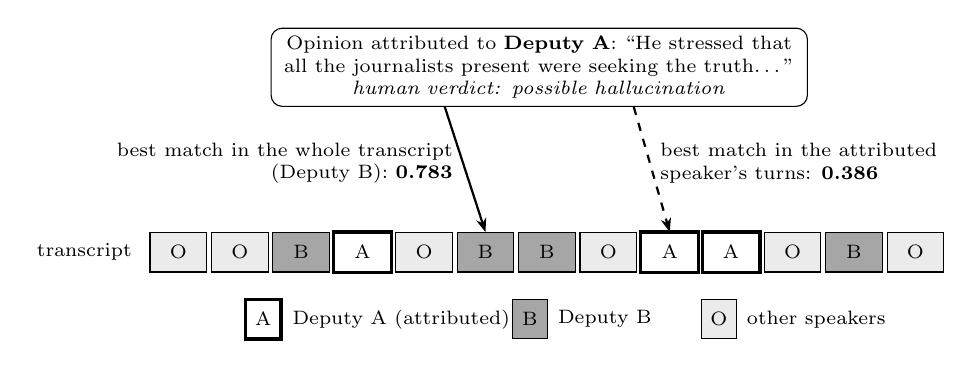
\begin{tikzpicture}[x=1cm,y=1cm,font=\scriptsize,
  seg/.style={draw,minimum height=0.5cm,minimum width=0.72cm,inner sep=0pt,anchor=west},
  arr/.style={-{Stealth[length=5pt]},thick}]
\foreach \i/\t/\f in {0/O/black!8,1/O/black!8,2/B/black!35,3/A/white,
    4/O/black!8,5/B/black!35,6/B/black!35,7/O/black!8,8/A/white,9/A/white,
    10/O/black!8,11/B/black!35,12/O/black!8}{
  \node[seg,fill=\f] (s\i) at (\i*0.78,0) {\t};
}
\foreach \i in {3,8,9}{\draw[very thick] (s\i.south west) rectangle (s\i.north east);}
\node[anchor=east] at (-0.1,0) {transcript};
\node[draw,rounded corners,fill=white,text width=6.6cm,align=center,inner sep=3pt]
  (op) at (4.95,2.35) {Opinion attributed to \textbf{Deputy A}: ``He stressed that
  all the journalists present were seeking the truth\ldots''\\
  \emph{human verdict: possible hallucination}};
\draw[arr] (op.south) ++(-1.2,0) -- node[left,align=right,pos=.45]
  {best match in the whole transcript\\(Deputy B): \textbf{0.783}} (s5.north);
\draw[arr,dashed] (op.south) ++(1.2,0) -- node[right,align=left,pos=.45]
  {best match in the attributed\\speaker's turns: \textbf{0.386}} (s8.north);
% legend
\node[seg,fill=white,very thick,minimum width=0.45cm] (l1) at (1.2,-0.85) {A};
\node[anchor=west] at (l1.east) {Deputy A (attributed)};
\node[seg,fill=black!35,minimum width=0.45cm] (l2) at (4.6,-0.85) {B};
\node[anchor=west] at (l2.east) {Deputy B};
\node[seg,fill=black!8,minimum width=0.45cm] (l3) at (7.0,-0.85) {O};
\node[anchor=west] at (l3.east) {other speakers};
\end{tikzpicture}
\caption{A misattribution from the dataset (participants pseudonymised). The order of
turns in the strip is schematic; the two similarity scores are measured. A
score computed over the whole transcript finds strong support ($0.783$), but
that support comes from another deputy (Deputy B). Restricted to the attributed speaker's
turns, the best match drops to $0.386$.}
\label{fig:incidencia}
\end{figure}

Our starting observation is that the best match may belong to the wrong
person. Figure~\ref{fig:incidencia} shows a real case, with the participants
pseudonymised. In a hearing on press
freedom, the summary attributes to Deputy~A the opinion
``\emph{Destacou que todos os jornalistas presentes estavam em busca da
verdade, independentemente de suas prefer\^encias pol\'iticas}'' (``He
stressed that all the journalists present were seeking the truth, regardless
of their political preferences''), and the human annotator marked it as not
supported (a possible hallucination under the annotation protocol). The most similar sentence in the transcript has a cosine similarity
of $0.783$, but it was spoken by Deputy~B. The most similar
sentence among Deputy~A's own turns scores $0.386$ and concerns a different
point. A score computed over the whole transcript sees a well-supported
opinion; a score computed over the attributed speaker's turns sees an
unsupported one. This case motivates a structural limitation (Section~\ref{sec:auditoria}):
when sentence scores omit speaker identity, any score that combines sentence-level
scores through a maximum, a mean or a similar function ignores which speaker
produced each sentence, and therefore cannot separate the two situations
(Observation~\ref{prop:incidencia}).

This observation raises two central questions, which organise the paper.
The first question is how much conditioning on the speaker helps, and at what cost. We compare
the opinion with the attributed speaker's turns and with the other speakers'
turns, and use these comparisons as features. We call them
\emph{speaker-incidence features}, because they use which speaker uttered
each sentence. The best match in the attributed speaker's turns alone raises
the AUROC from $0.57$ to $0.75$, and a logistic regression on all the features
reaches $0.76$, without LLM-judge calls.
The second question is how such an inexpensive detector should be combined with the
costly committee of judges. The usual approach fits a model, such as a logistic regression, on
the judges' votes and the new features together. On this dataset it does not
improve the committee: its AUROC falls below the committee's in 19 of 20
random assignments of hearings to folds. The reason is structural: the
committee's vote count takes only thirteen values, so many opinions are tied,
and a second detector could usefully order them. A weighted sum, however, does
more than order the ties: it can also reverse two opinions that the committee
orders correctly, whenever the new detector disagrees strongly enough
(Proposition~\ref{prop:soma}). We instead rank opinions by the committee's
vote count and use the new detector only to order opinions that received the
same count. This \emph{lexicographic} combination preserves every strict committee
ordering, and its gain is given by an exact formula
(Proposition~\ref{thm:lex}) that depends on two quantities: how often the
committee cannot order a pair of opinions, and how well the new detector
orders those pairs. Both can be estimated on a labelled sample before the
combination is deployed, and together they indicate where the rule pays off:
its gain is largest when judges are few, which is where it saves the most
calls.

\begin{figure}[t]
\centering
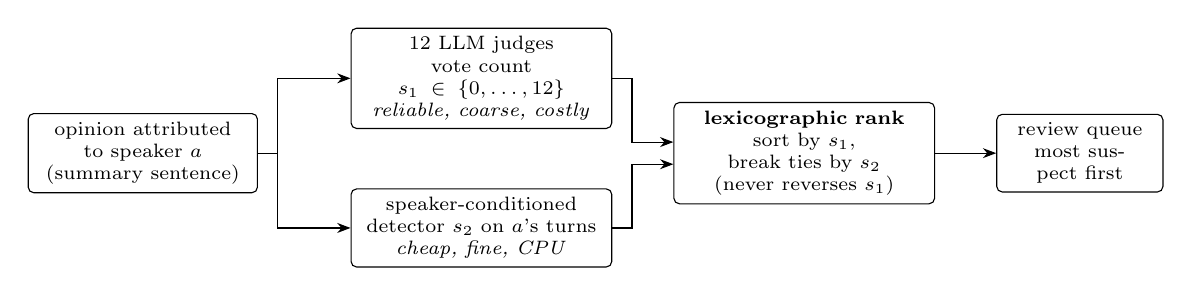
\begin{tikzpicture}[font=\scriptsize, >=Stealth,
  box/.style={draw, rounded corners=2pt, align=center, inner sep=3pt, text width=2.7cm},
  wide/.style={draw, rounded corners=2pt, align=center, inner sep=3pt, text width=3.1cm}]
  \node[box] (op) at (0,0) {opinion attributed to speaker $a$\\(summary sentence)};
  \node[wide] (j) at (4.3,0.95) {12 LLM judges\\vote count $s_1\in\{0,\dots,12\}$\\\emph{reliable, coarse, costly}};
  \node[wide] (d) at (4.3,-0.95) {speaker-conditioned detector $s_2$ on $a$'s turns\\\emph{cheap, fine, CPU}};
  \node[wide] (l) at (8.4,0) {\textbf{lexicographic rank}\\sort by $s_1$, break ties by $s_2$\\(never reverses $s_1$)};
  \node[box, text width=1.9cm] (q) at (11.9,0) {review queue\\most suspect first};
  \draw[->] (op.east) -- ++(0.25,0) |- (j.west);
  \draw[->] (op.east) -- ++(0.25,0) |- (d.west);
  \draw[->] (j.east) -- ++(0.25,0) |- ([yshift=4pt]l.west);
  \draw[->] (d.east) -- ++(0.25,0) |- ([yshift=-4pt]l.west);
  \draw[->] (l.east) -- (q.west);
\end{tikzpicture}
\caption{Overview of the method. The detector reads the attributed speaker's
turns and is used only to order opinions the judges cannot order.}
\label{fig:visao}
\end{figure}

\needspace{4\baselineskip}
\medskip\noindent\textbf{Contributions.}
\begin{itemize}
  \itemsep1pt
  \item Speaker-incidence features, motivated by the observation that pooled
    verification scores ignore speaker attribution. They raise AUROC from
    $0.57$ to $0.76$ at no LLM cost (measured CPU time in Section~\ref{sec:custo}), and an audit of 50 positives finds
    that about a quarter were classified as misattributions of this kind
    (Sections~\ref{sec:teoria-incidencia} and~\ref{sec:res-orador}).
  \item A rule for combining a reliable but coarse detector with an
    inexpensive but finer one. The rule preserves the reliable detector's
    strict orderings, and an elementary decomposition of AUROC gives its gain
    exactly (Section~\ref{sec:fusao}). Estimated on one half of the
    hearings, the decomposition forecasts the average gain on the other half
    using development data alone (Section~\ref{sec:res-escada}).
  \item A reduction in the number of LLM calls needed for a given accuracy.
    The rule raises each single judge by $0.046$ to $0.101$ AUROC, and in an
    exploratory analysis eight judges with the rule are non-inferior to the
    full committee of twelve. With the best single judge, a reviewer who
    checks the $10\%$ most suspect opinions finds $52.2\%$ of the
    hallucinations instead of $40.5\%$
    (Sections~\ref{sec:res-escada} and~\ref{sec:res-fila}).
  \item A characterisation of what remains: on the pairs of opinions that the
    committee orders incorrectly, the inexpensive detector performs below
    chance, so rules that overrule the committee when the two disagree
    did not robustly recover the remaining gap in our experiments
    (Section~\ref{sec:res-orcamento}).
  \item A reproducible evaluation including negative results
    (Section~\ref{sec:negativos}) and simple, untrained tie-breaking controls;
    all code is available.\footnote{\url{https://github.com/caua-sathler/IdeiasEmRede-TopoIA}}
\end{itemize}

% =============================================================================
\section{Related Work}
\label{sec:relacionados}

\paragraph{Hallucination detection and LLM judges.}
\citet{publichearingbr} introduce the corpus, the human verdicts and the
twelve LLM-judge annotations used here. \citet{maynez2020faithfulness}
propose the standard taxonomy of faithfulness errors in abstractive
summarisation. The error our features target, content attributed to the wrong
speaker, is identified in dialogue summarisation by
\citet{ramnath2026dialsummer}, who report that LLM judges detect it only
moderately well. \citet{zheng2023judging} study the reliability of LLM judges,
including position, verbosity and self-preference biases.
Importantly, the original PublicHearingBR verification pipeline already
retrieves four chunks from the attributed person's speech. Our contribution
is to quantify inexpensive incidence signals against pooled baselines and
controls, and to use them to refine the released judges' coarse rankings.
The cosine/NLI features and the released judges differ in both evidence
selection and scoring; conditioning is isolated by comparing each feature
with its own unconditioned counterpart.

\paragraph{Combining detectors.} The question of when a classifier should
abstain goes back to \citet{chow1970optimum}, with the risk--coverage
formalism of \citet{elyaniv2010foundations}. A coarse detector abstains
implicitly when it assigns the same score to two items, and
Lemma~\ref{lem:contab} quantifies the effect of these ties on AUROC. Ensemble methods usually combine scores by weighted sums; the
decomposition of AUROC into tied and separated pairs that we use is elementary,
and its value is practical.

% =============================================================================
\section{Background}
\label{sec:background}

\subsection{AUROC and tied pairs}
\label{sec:auroc-pairwise}
An \emph{opinion} is a generated summary statement attributed to a named
participant. We call the official unsupported labels \emph{positives} or
\emph{possible hallucinations}, and the supported labels \emph{negatives}.
These names refer to the four-chunk annotation protocol, not a new judgement
of the full transcript. A detector assigns a score $s$, with larger values
indicating greater suspicion.

\begin{definition}[AUROC]\label{def:auroc}
For independently and uniformly sampled positive and negative opinions
$p\in P$, $n\in N$, the Area Under the Receiver Operating Characteristic
Curve is the Mann--Whitney statistic \citep{hanley1982meaning}:
\begin{equation}\label{eq:auroc}
\AUC(s)=\Pr[s(p)>s(n)]+\tfrac12\Pr[s(p)=s(n)].
\end{equation}
\end{definition}
AUROC counts correctly ordered positive--negative pairs, giving half credit
to ties. Chance is $0.5$ and perfect ranking is $1$. Unlike accuracy, it
cannot reward a detector simply for predicting the majority class, which
covers $88.1\%$ of this dataset. It is invariant to strictly increasing
transformations of a score. We complement it with recall at fixed review
budgets (Section~\ref{sec:res-fila}).

\begin{lemma}[Tie accounting]\label{lem:contab}
Let $A(s)=\Pr[s(p)>s(n)]$ and $\tau(s)=\Pr[s(p)=s(n)]$. Then
$\AUC(s)=A(s)+\tau(s)/2\le 1-\tau(s)/2$, with equality exactly when all
separated pairs are correctly ordered.
\end{lemma}
\begin{proof}
Equation~\eqref{eq:auroc} gives the identity; $A(s)\le1-\tau(s)$ gives the
bound. This standard accounting identity is not a contribution.\qedhere
\end{proof}

\subsection{Pooled scores and rankings with ties}
\label{sec:bg-preorder}
A pooled verifier combines sentence scores $f(o,u_i)$ using a maximum,
mean or top-$k$ mean. If those scores omit speaker identity, their aggregate
cannot recover it. We write $T$ for the transcript, $T_a$ for the sentences
spoken by participant $a$, and $\sigma$ for the sentence-to-speaker map.

\begin{definition}[Detector preorder]\label{def:preorder}
A real-valued score induces a \emph{total preorder}
$x\preceq_s y\iff s(x)\le s(y)$: a reflexive, transitive ranking in which
all items are comparable and ties are allowed. Write $x\approx_s y$ for a
tie and $x\prec_s y$ for strict order. Its equivalence classes are the
groups of equal scores. A refinement preserves all strict orders and may
split ties. All preorders below are total and induced by scores.
\end{definition}
The primary score $s_1$ is a judge vote or committee vote count, the
secondary score $s_2$ an inexpensive detector. We use $\tau$ for the
primary tied-pair fraction and $\alpha$ for the secondary AUROC restricted
to those positive--negative pairs. Their product determines the gain of
breaking ties, as shown next.

% =============================================================================
\section{Theory}
\label{sec:teoria}

\subsection{Pooled scores ignore the speaker}
\label{sec:teoria-incidencia}

Fix an opinion $o$ attributed to speaker $a$, a transcript
$T = (u_1, \dots, u_m)$ with a speaker map $\sigma : T \to \mathcal{A}$ that
assigns each sentence to the participant who uttered it, and any
sentence-level score $f(o, u_i)$.

\begin{observation}[Incidence blindness]
\label{prop:incidencia}
Any pooled score $G\bigl(\{f(o,u_i)\}_i\bigr)$, where $G$ is a maximum, a
mean, a top-$k$ mean or any other permutation-invariant function, is
invariant under every reassignment of the speaker map $\sigma$. Consequently,
no such score can distinguish an opinion supported by the turns of its
attributed speaker from the same opinion supported only by the turns of other
speakers.
\end{observation}

\begin{proof}
$G$ does not receive $\sigma$ as an argument. For a concrete separation, take
two sentences with scores $0.9$ and $0.1$. Under $\sigma_1$ the first sentence
belongs to $a$; under $\sigma_2$ it belongs to some $b \neq a$. Every pooled
$G$ takes the same value on both configurations, but only the first one
supports the opinion as attributed. \qedhere
\end{proof}

Equivalently, exchanging the speaker labels of all turns in a hearing
leaves every pooled score unchanged, although it changes the answer to the
question of whether the attributed person said what the opinion claims. No
choice of pooling function avoids this. The remedy is to pool over the
attributed speaker's sentences $T_a = \sigma^{-1}(a)$ instead of the whole
transcript, and to compare the result with the other speakers' sentences.
Section~\ref{sec:res-orador} shows that this restriction raises AUROC by
$0.18$, and that additional features describing how the support is
distributed across speakers add a smaller, significant improvement.

\subsection{Combining a coarse and a fine detector}
\label{sec:fusao}

Consider a \emph{reliable but coarse} detector $s_1$, such as the committee,
which is accurate when it separates two items but assigns the same value to
many of them, and an \emph{inexpensive but fine} detector $s_2$, which
separates almost all items but is less accurate. We call $s_1$ the
\textbf{primary} and $s_2$ the \textbf{secondary} detector throughout. The
standard way to combine them is a weighted sum, or a logistic regression on
both scores, which we call \emph{stacking}.

\begin{proposition}[A weighted sum can reverse the primary detector]
\label{prop:soma}
Let $w_1,w_2>0$ and let $x \prec_1 y$, that is, $s_1(x)<s_1(y)$. The weighted
sum reverses this pair, $w_1 s_1(x)+w_2 s_2(x) > w_1 s_1(y)+w_2 s_2(y)$, if
and only if $s_2(x)-s_2(y) > (w_1/w_2)\bigl(s_1(y)-s_1(x)\bigr)$.
Consequently, a sufficiently large ratio $w_2/w_1$ reverses some strict
relation of $\prel_1$ if and only if the two detectors disagree on some pair,
that is, $s_1(x)<s_1(y)$ and $s_2(x)>s_2(y)$ for some items $x,y$.
\end{proposition}

\begin{proof}
The first claim rearranges the inequality. If $s_1(x)<s_1(y)$ and
$s_2(x)>s_2(y)$, the condition holds for every ratio
$w_2/w_1 > \bigl(s_1(y)-s_1(x)\bigr)/\bigl(s_2(x)-s_2(y)\bigr)$. Conversely,
if a pair with $s_1(x)<s_1(y)$ is reversed, the condition gives
$s_2(x)>s_2(y)$. \qedhere
\end{proof}

To correct a pair that the committee orders wrongly, a secondary detector
must disagree with the committee on that pair. A weighted sum that gives it
enough weight acts on every such disagreement, and therefore also overturns
decisions that the committee got right.

\begin{example}[A concrete reversal]
\label{ex:witness}
Consider three opinions. Let $s_1$ be the committee's vote count divided by
twelve and $s_2$ an inexpensive score in $[0,1]$, with equal weights.
\begin{center}\small
\begin{tabular}{lccc l}
\toprule
 & $x$ & $y$ & $z$ & \\
\midrule
committee $s_1$ & $4/12$ & $5/12$ & $5/12$ & $x \prec_1 y \approx_1 z$ \\
inexpensive score $s_2$ & $0.95$ & $0.10$ & $0.90$ & \\
\midrule
sum $s_1 + s_2$ & $1.28$ & $0.52$ & $1.32$ & \textbf{reverses} $x \prec_1 y$ \\
lexicographic   & $(4/12,\,0.95)$ & $(5/12,\,0.10)$ & $(5/12,\,0.90)$ & keeps $x \prec y \prec z$ \\
\bottomrule
\end{tabular}
\end{center}
The sum ranks $x$ (four votes) above $y$ (five votes) because the inexpensive
score disagrees with the committee. The lexicographic order keeps the
committee's decision and uses $s_2$ only to separate $y$ from $z$, which the
committee could not order.
\end{example}

\begin{definition}[Lexicographic combination]
\label{def:lex}
Given total detector preorders $\prel_1$ and $\prel_2$,
\begin{equation}
  \label{eq:lex}
  x \lex y \quad :\Longleftrightarrow\quad
  x \prec_1 y \quad\text{or}\quad \bigl(x \approx_1 y \ \text{and}\
  x \prel_2 y\bigr).
\end{equation}
Operationally: rank items by $s_1$, and within each group of items with equal
$s_1$, rank them by $s_2$.
\end{definition}

\begin{proposition}[Lexicographic combination]
\label{thm:lex}
$\lex$ is a total preorder containing $\prel_1 \cap \prel_2$, and
\begin{enumerate}
  \itemsep1pt
  \item[(i)] it never reverses a strict relation of $\prel_1$: if
    $x \prec_1 y$, then $x \prec_{\mathrm{lex}} y$;
  \item[(ii)] it refines $\prel_1$ only within its equivalence classes, and
    uses no other information;
  \item[(iii)] if $\alpha$ denotes the AUROC of $s_2$ \emph{restricted to the
    positive--negative pairs that $\prel_1$ ties} (set $\alpha=1/2$ if $\tau=0$), then
    \begin{equation}
      \label{eq:captura}
      \AUC(\lex) \;=\; \AUC(s_1) \;+\; \tau(s_1)\bigl(\alpha - \tfrac12\bigr)
      \qquad\text{exactly.}
    \end{equation}
    The combination therefore recovers the fraction $2\alpha - 1$ of the
    maximum possible gain $\tau/2$. It attains the full $\tau/2$ if and only
    if $\alpha = 1$, and in all cases
    $\AUC(\lex) \in [\AUC(s_1) - \tau/2,\ \AUC(s_1) + \tau/2]$.
\end{enumerate}
\end{proposition}

In words, the gain equals the share of tied pairs times how much better than
a coin flip the secondary detector orders them.

\begin{proof}
Totality and transitivity of \eqref{eq:lex} follow directly from the
definition. For the inclusion, let $x \prel_1 y$ and $x \prel_2 y$: either
$x \prec_1 y$ and the first clause applies, or $x \approx_1 y$ and the second
applies. Claim (i) is the first clause, and claim (ii) the second. For (iii),
let $A = A(s_1)$, so that $\AUC(s_1) = A + \tau/2$ by Lemma~\ref{lem:contab}.
By (i), the pairs that $s_1$ separates are ordered in the same way by $\lex$
and contribute $A$. By (ii), the tied pairs, of total probability $\tau$, are
ordered by $s_2$ alone; applying Definition~\ref{def:auroc} to this
sub-population, they contribute $\tau \alpha$ instead of $\tau/2$. Hence
$\AUC(\lex) = A + \tau \alpha$, and subtracting $\AUC(s_1)$ gives
\eqref{eq:captura}. The bound follows from $\alpha \in [0,1]$. \qedhere
\end{proof}

\begin{remark}[The gain depends on $\alpha$, not on the global AUROC of $s_2$]
\label{rem:orcamento}
By Proposition~\ref{thm:lex}(i), the lexicographic combination keeps every
pair that $s_1$ separates in the order $s_1$ gives it. The pairs that $s_1$
orders wrongly, which account for the gap $1-\tau/2-\AUC(s_1)$, are therefore
out of its reach, and for any secondary detector the change in AUROC lies
within $\pm\tau/2$. Within this range, Equation~\eqref{eq:captura} involves
only two quantities: $\tau$, which depends on the primary detector and the
labels but not on $s_2$, and $\alpha$, the AUROC of $s_2$ on the tied pairs.
The AUROC of $s_2$ on the whole task does not appear. Two practical
consequences follow. First, a candidate secondary detector should be
evaluated on the primary detector's ties rather than on the whole task: our
features reach $0.78$ overall but only $\alpha = 0.59$ on the committee's
ties. Second, the maximum gain $\tau/2$ can be computed before any secondary
detector is built, and once $\alpha$ is estimated on a development set the
gain follows without running the combination.
Section~\ref{sec:res-escada} tests this forecast on unseen hearings.
\end{remark}

\begin{remark}[From the lexicographic combination to the weighted sum]
\label{rem:portao}
Let $r_1(x)\in\{1,\dots,K\}$ index the primary score's classes, and
$r_2(x)\in[0,1]$ be the secondary score's normalised rank. The score
$f_\gamma=r_1+\gamma r_2$ induces the lexicographic order for every
$0<\gamma<1$: the secondary term cannot bridge the unit gap between
primary classes. At $\gamma=1$, extreme adjacent items may tie; for
$\gamma>1$, some primary orders may reverse. Thus lexicographic tie-breaking
can also be implemented as a bounded additive perturbation, without
selecting a weight on the evaluation labels. Section~\ref{sec:res-orcamento}
examines whether allowing reversals helps empirically.
\end{remark}

% =============================================================================
\section{Data and Methods}
\label{sec:dados}

This section describes the data, the statistical protocol shared by all
experiments, the speaker-incidence features, and the two detectors combined
in Section~\ref{sec:res-fusao}.

\paragraph{Data.} We use all 206 hearings of PublicHearingBR: $4{,}238$
generated opinions with human NLI annotations (504 positive, $11.9\%$)
and stored votes from four models with three prompts each. Both human and
LLM verdicts concern the four chunks retrieved by the original
speaker-conditioned pipeline. Our features instead access the transcript
sentences and recovered speaker turns. Sentences and opinions are embedded
with \texttt{paraphrase-multilingual-mpnet-base-v2} \citep{reimers2019sbert}. A \emph{turn} is a block of consecutive sentences
spoken by one participant. Turns are recovered from the transcript's speaker
markers (\texttt{O SR.\ NAME --}): each sentence is assigned to the most
recent marker. The participant named in the summary is
matched to a turn speaker by overlap of name tokens. The match succeeds for
$85.7\%$ of the opinions ($n = 3{,}630$, 408 positive), which form the main
evaluation set, since both the speaker-incidence features and the combination
experiments require the attributed speaker's turns. A failed match is itself
informative and is used as a feature in Section~\ref{sec:res-orador}.
Entailment probabilities come from mDeBERTa-v3-base-xnli
\citep{laurer2024less}, a natural language inference (NLI) model that scores whether a premise entails a hypothesis; each sentence pair evaluated is one \emph{NLI call}.

\paragraph{Statistical protocol.} All learned models are evaluated \emph{out of fold}: we use five-fold
cross-validation in which all opinions of a hearing fall in the same fold
(\texttt{GroupKFold}), so each opinion is scored by a model fitted on other
hearings and no model is evaluated on data it was fitted on. Models are logistic regressions with balanced class weights and
$C=1$; features are standardised using only each training fold.
Confidence intervals resample whole hearings rather than opinions, since
opinions from the same transcript are not independent ($3{,}000$ to $5{,}000$
bootstrap resamples, depending on the analysis; all intervals are $95\%$ and, when two detectors are
compared, paired on the same resamples). Two additional sources of variance
are controlled in the combination experiments. A random tie-break is itself a
random variable, so we compare against $200$ random draws. The assignment of
hearings to folds is not captured by the bootstrap, so the main combination comparison is
repeated over $20$ random assignments of hearings to folds (\emph{fold
partitions}) and reported as median and range. Where a single value is
reported, it comes from the deterministic five-fold reference partition.
Feature-only models and combination models use the explicitly specified
feature sets below. We report negative findings alongside positive ones;
research hypotheses and their provenance are archived in
\texttt{code/predictions/}.

\paragraph{Speaker-incidence features.} For an opinion $o$ attributed to the
matched speaker $a$, let $S(o,\cdot)$ be the cosine similarity between $o$ and
each transcript sentence, $T$ the set of all sentences, and $T_a$ the set of
sentences spoken by $a$.

\begin{center}
\small
\begin{tabular}{@{}lp{0.72\linewidth}@{}}
\toprule
$\mathrm{cos}_g$ & $\max_{s \in T} S(o,s)$: best match in the whole transcript (baseline) \\
$\mathrm{cos}_s$ & $\max_{s \in T_a} S(o,s)$: best match in the attributed speaker's turns \\
$\Delta$ & $\max_{b \neq a}\max_{s \in T_b} S(o,s) - \mathrm{cos}_s$: how much
  better another speaker supports the opinion \\
$\mathrm{share}_a$ & sum of the similarities of the ten best global matches
  that lie in $T_a$, divided by their total \\
$\mathrm{rank}_a$ & rank of $a$ among all speakers ordered by their best
  match, scaled to $[0,1]$ \\
$\mathrm{cover}_a$ & $1$ if $a$ is among the strong supporters, i.e.\ the
  speakers with at least one sentence of similarity $\ge 0.65$ \\
$n_{\rm sup}$, $n_{\rm op}$ & number of speakers with similarity $\ge0.65$;
  number of opinions attributed to the matched speaker in the hearing \\
$\mathrm{nli}_s, \mathrm{nli}_g$ & maximum entailment probability over the
  five best-matching sentences of $a$ / of the whole transcript \\
\bottomrule
\end{tabular}
\end{center}

The feature $\mathrm{cos}_s$ asks whether the attributed speaker's own turns
support the opinion, and $\Delta$ asks whether somebody else supports it
better; we call $\Delta$ the \emph{misattribution score}. When a feature is
used alone as a detector, it is oriented so that larger values indicate a
more suspect opinion (for example, $-\mathrm{cos}_s$). The remaining
features describe how much of the support belongs to the attributed speaker,
where that speaker ranks, and whether the speaker is among the supporters at
all. None of these quantities can be computed from a pooled score
(Observation~\ref{prop:incidencia}). The cosine features require no model call
beyond the precomputed embeddings; the two entailment features require ten
NLI calls per opinion. NLI uses the top five cosine matches in each pool,
with premise and hypothesis truncated to 280 characters and paired inputs
to 192 tokens. The cosine regression uses
$(\mathrm{cos}_s,\mathrm{best}_{\rm other},\mathrm{share}_a,n_{\rm sup},
\mathrm{cover}_a,\mathrm{rank}_a)$; the NLI variant adds
$(\mathrm{nli}_s,\mathrm{nli}_g,\mathrm{nli}_g-\mathrm{nli}_s)$.
Combination experiments additionally include $n_{\rm op}$, explaining the
small difference from feature-only AUROCs.

\paragraph{The two detectors combined in Section~\ref{sec:res-fusao}.} The
primary detector $s_1 \in \{0,\dots,12\}$ is the number of judges that flag
an opinion. This unweighted vote count outperforms logistic weights fitted
out of fold on the same votes ($0.9260$ vs.\ $0.9245$ on the representative
partition, and a median of $0.9226$ over twenty partitions,
Table~\ref{tab:estab}). The secondary detector is a logistic regression on all the
speaker-incidence features, including NLI and $n_{\rm op}$ ($0.7787$, up to ten NLI
calls per opinion); unless stated otherwise, Section~\ref{sec:res-fusao} uses
this detector. \emph{Stacking}
denotes a logistic regression fitted out of fold on the votes and the same
features together. As a control, Section~\ref{sec:res-controles}
also uses a deliberately weak inexpensive detector, $\mathrm{cos}_g$.

% =============================================================================
\section{Results I: Speaker-Incidence Features}
\label{sec:res-orador}

\subsection{Conditioning on the attributed speaker}

Table~\ref{tab:orador} reports the main result of this section. On the
$3{,}630$ matched opinions, the best match in the whole transcript reaches an
AUROC of $0.5676$ ($0.5628$ over all $4{,}238$ opinions). Computing the same
similarity over the attributed speaker's turns raises it to $0.7455$, a
difference of $+0.178$ (clustered CI $[+0.128, +0.237]$).

\begin{table}[!ht]
  \centering
  \caption{AUROC of each signal against the human verdict on the
  matched-speaker subset ($n=3{,}630$, 408 positives). ``0 calls'' means the
  signal is computed from precomputed embeddings and speaker markers alone.}
  \label{tab:orador}
  \small
  \begin{tabular}{@{}llc@{}}
    \toprule
    \textbf{Signal} & \textbf{Cost / opinion} & \textbf{AUROC} \\
    \midrule
    $\mathrm{cos}_g$: best match in the whole transcript (baseline) & 0 calls & 0.5676 \\
    $\mathrm{nli}_g$: best entailment in the whole transcript (baseline) & up to 5 NLI & 0.5828 \\
    \midrule
    $\mathrm{cos}_s$: \textbf{best match in the attributed speaker's turns} & 0 calls & \textbf{0.7455} \\
    $\Delta$: misattribution score                                & 0 calls & 0.7595 \\
    $\mathrm{share}_a$: share of the support                     & 0 calls & 0.7135 \\
    $\mathrm{rank}_a$: rank of the speaker                       & 0 calls & 0.7258 \\
    $\mathrm{cover}_a$: speaker among strong supporters          & 0 calls & 0.6706 \\
    \textbf{all speaker-incidence features, out of fold}          & 0 calls & \textbf{0.7605} \\
    all features $+$ $\mathrm{nli}_s, \mathrm{nli}_g$            & $\sim$10 NLI & \textbf{0.7792} \\
    \bottomrule
  \end{tabular}
\end{table}

Three controls address alternative explanations.
\textbf{Speaker identity.} Computing the same feature over a \emph{randomly
chosen other} speaker of the same hearing, matched for number of turns, gives
$0.5209$, which is at chance and below the global baseline. The paired
difference between the attributed and the random speaker is $+0.2246$
$[+0.1903, +0.2592]$, so the signal comes from \emph{who} spoke, not from how
much. \textbf{Number of sentences.} The number of sentences of the attributed
speaker alone scores $0.4953$ (correlation $+0.26$ with $\mathrm{cos}_s$), so
the effect is not an artefact of taking a maximum over fewer sentences.
\textbf{Features beyond the single score.} Out of fold, the full set of
features improves on the best single conditioned score, from $0.7447$ to
$0.7605$, a paired difference of $+0.0159$ $[+0.0028, +0.0298]$.
Additionally, two complementary findings emerge from the data: first, a failed speaker match is informative
(hallucination rate $15.8\%$ vs.\ $11.2\%$), and using it as an indicator feature extends
the detector to all $4{,}238$ opinions ($0.7435$ out of fold); second,
conditioning on the speaker also benefits entailment, where $\mathrm{nli}_s$ improves on
$\mathrm{nli}_g$ by $+0.1264$ $[+0.0928,+0.1614]$. Contrary to our hypothesis, however, $\mathrm{nli}_s$ alone ($0.7095$) does not outperform
$\mathrm{cos}_s$ ($0.7455$); entailment adds value only in combination with
the cosine features ($+0.0186$ $[+0.0060,+0.0309]$).

\subsection{Comparison and combination with individual judges}

The twelve judges each emit a binary vote and reach an AUROC between $0.7340$
and $0.8468$. Without LLM-judge calls, the speaker-incidence features
($0.7605$) outperform the three weakest judges ($0.7340$, $0.7401$, $0.7522$).
Combined with any single judge by \emph{rank sum}, which adds the two ranks
and requires no fitting, they improve that judge in twelve cases out of
twelve, with every clustered CI excluding zero. The gains range from $+0.027$
to $+0.094$, are largest for the weakest judges (per-judge results are in the
repository), and the best such rank-sum combination reaches $0.8823$.
Section~\ref{sec:res-escada} reports the lexicographic combination, which
performs better.
Section~\ref{sec:res-fusao} examines the full twelve-judge committee and how
to combine the features with it without degrading it.

\paragraph{Interpretation.} One type of error these features detect has a
simple description: a plausible hallucination that is on topic for the
hearing but not for the turns of the person to whom it is attributed. A global similarity
score cannot see this difference (Observation~\ref{prop:incidencia}), whereas
the speaker-conditioned features are built to capture it. That the strongest
single feature is the misattribution score $\Delta$ ($0.7595$) is consistent
with this interpretation. The example of Figure~\ref{fig:incidencia}
($0.783$ in the whole transcript, $0.386$ in the attributed speaker's turns,
$\Delta=+0.40$) is one such case: its misattribution score exceeds that of $99.3\%$ of the
grounded opinions, in agreement with the human verdict. Section~\ref{sec:auditoria} measures how common this type
of error is among the positives.

\subsection{What kind of error are the positives?}
\label{sec:auditoria}

We examined a random sample of 50 of the 408 benchmark positives
(seed 20260923) with two Claude annotation passes, using retrieved
speaker-specific and global evidence with neighbouring sentences.
The model annotations agree on 45 items (Cohen's $\kappa=0.81$).
Both assign 12 items ($24\%$) to misattribution, 30 to apparent support by
the attributed speaker and 3 to distortion; five disagreements are left
unresolved. All 12 consensus misattributions have positive $\Delta$
(mean $0.21$). Apparent support outside the official retrieval context is
consistent with the benchmark's four-chunk scope. This exploratory audit
characterises the error mechanisms without replacing the official labels.
Sampling, category assignments and the protocol are provided in
\texttt{code/AUDIT\_PROTOCOL.md}.

% =============================================================================
\section{Results II: Combining the Features with the Committee}
\label{sec:res-fusao}

\subsection{How the committee's ties are distributed}

The sum of the twelve votes takes thirteen values and reaches an AUROC of
$0.9260$. The ranking it induces is nevertheless coarse: $\tau = 4.65\%$ of
positive--negative pairs are tied, so by Lemma~\ref{lem:contab} the largest
possible gain from ordering them is $\tau/2 = 0.0232$, and a perfect
secondary detector would reach $0.9492$ (not the bound $1-\tau/2 = 0.9768$ of
Lemma~\ref{lem:contab}, which would also require the committee to order all
separated pairs correctly). This does not mean that the judges
are close to a performance ceiling: their
sensitivity ranges from $0.48$ to $0.92$ and their specificity from $0.64$ to
$0.99$, and two of them miss more than half of the hallucinations while lying within
$0.009$ of their own bound $1-\tau/2$. All
gains reported below are bounded by $\tau/2$, not by that larger gap.

\begin{figure}[!ht]
\centering
% Coordinates generated by code/src/committee_histogram.py. Do not edit by
% hand: rerun the script and paste.
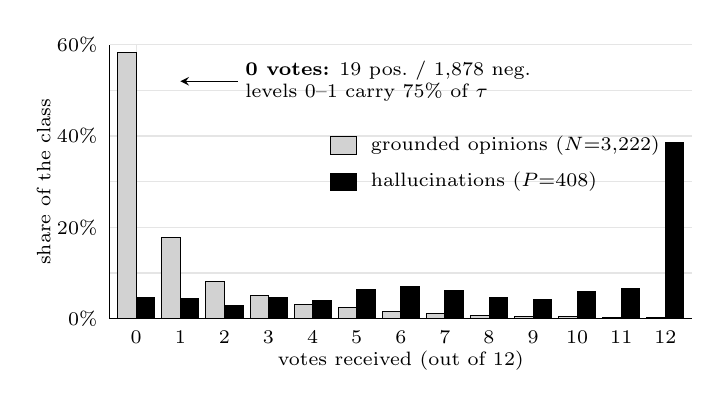
\begin{tikzpicture}[x=0.56cm, y=0.058cm, font=\scriptsize]
  \draw[gray!20] (-0.6,0) grid[xstep=20, ystep=10] (12.6,60);
  \draw (-0.6,0) -- (12.6,0);  \draw (-0.6,0) -- (-0.6,60);
  \foreach \k in {0,...,12} \node[below=1pt] at (\k,0) {\k};
  \foreach \yy in {0,20,40,60} \node[left=1pt] at (-0.6,\yy) {\yy\%};
  \node[below=8pt] at (6,0) {votes received (out of 12)};
  \node[rotate=90] at (-2.1,30) {share of the class};
  % negatives: grey; positives: black
  \foreach \k/\h in {0/58.3,1/17.8,2/8.1,3/5.1,4/3.2,5/2.5,6/1.6,7/1.1,8/0.8,9/0.5,10/0.4,11/0.2,12/0.3}
    \draw[fill=gray!35, line width=0.3pt] (\k-0.42,0) rectangle (\k,\h);
  \foreach \k/\h in {0/4.7,1/4.4,2/2.9,3/4.7,4/3.9,5/6.4,6/7.1,7/6.1,8/4.7,9/4.2,10/5.9,11/6.6,12/38.5}
    \draw[fill=black, line width=0.3pt] (\k,0) rectangle (\k+0.42,\h);
  \node[anchor=west, align=left, inner sep=1pt] at (2.4,52)
    {\textbf{0 votes:} 19 pos.\ / 1,878 neg.\\
     levels 0--1 carry $75\%$ of $\tau$};
  \draw[->, >=stealth] (2.3,52) -- (1.0,52);
  \fill[gray!35, draw=black, line width=0.3pt] (4.4,36) rectangle (5.0,40);
  \node[anchor=west] at (5.1,38) {grounded opinions ($N{=}3{,}222$)};
  \fill (4.4,28) rectangle (5.0,32);
  \node[anchor=west] at (5.1,30) {hallucinations ($P{=}408$)};
\end{tikzpicture}
\caption{The committee's tie structure. For each of the thirteen vote levels,
the share of grounded opinions (grey) and of hallucinations (black) receiving
that many votes. The tie fraction is $\tau=\sum_k \pi^+_k\pi^-_k$, the sum of
products of the two bars at each level: level~0 alone contributes $58\%$ of it
($\pi^-_0=0.583$, $\pi^+_0=0.047$), levels~0--1 contribute $75\%$.}
\label{fig:comite}
\end{figure}

Figure~\ref{fig:comite} explains why the tie fraction is small although half
of the opinions receive zero votes. The tie
fraction is a sum of \emph{products} of class shares. The zero-vote class
holds $58\%$ of the grounded opinions but only $4.7\%$ of the hallucinations
($19$ against $1{,}878$ opinions). Hallucinations rarely receive zero votes;
they concentrate at twelve votes ($38.5\%$), where almost no grounded opinion
is found.

\subsection{Decomposing the effect of each combination}
\label{sec:res-mecanismo}

Because AUROC is an average over pairs \eqref{eq:auroc}, it can be decomposed
exactly over any partition of the pairs. We divide the $1{,}314{,}576$
positive--negative pairs into those the committee \emph{separates}
($95.4\%$) and those it \emph{ties} ($4.6\%$), and measure the effect of each
combination on each group (Table~\ref{tab:mecanismo}).

\begin{table}[!ht]
  \centering
  \caption{Exact decomposition of AUROC over pair types.
  ``Reversals'' counts separated pairs whose order the fused score flips:
  \emph{harmful} if the committee had them right, \emph{benign} if wrong.
  One representative fold partition; stability is Table~\ref{tab:estab}.}
  \label{tab:mecanismo}
  \small
  \setlength{\tabcolsep}{5pt}
  \begin{tabular}{@{}lccc ccc@{}}
    \toprule
    & & \multicolumn{2}{c}{\textbf{contribution from}} &
      \multicolumn{3}{c}{\textbf{reversals among separated pairs}} \\
    \cmidrule(lr){3-4}\cmidrule(lr){5-7}
    \textbf{Method} & \textbf{AUROC} & separated & tied &
      total & harmful & benign \\
    \midrule
    committee (vote count) & 0.9260 & 0.9027 & 0.0232 & --- & --- & --- \\
    stacking (logistic)  & 0.9262 & 0.9013 & 0.0249 &
      \textbf{1.33\%} & 0.74\% & 0.59\% \\
    \textbf{lexicographic} & \textbf{0.9300} & 0.9027 & \textbf{0.0272} &
      \textbf{0.00\%} & 0.00\% & 0.00\% \\
    \bottomrule
  \end{tabular}
\end{table}

Tied pairs contribute exactly $\tau/2 = 0.0232$ to the committee's AUROC, as
Lemma~\ref{lem:contab} requires. The weighted combination (``stacking'')
extracts information from them, raising their contribution to $0.0249$
($+0.0017$), but it also reverses $1.33\%$ of the separated pairs, which costs
$0.0014$, so the net gain is $0.0002$. The lexicographic combination reverses
no pair and raises the contribution of the tied pairs to $0.0272$ ($+0.0040$).


\subsection{Main comparison}
\label{sec:res-principal}

Table~\ref{tab:estab} evaluates the combinations across twenty independent
\texttt{GroupKFold} partitions, supporting two main conclusions. First, stacking is worse than
the committee in median, and it is unstable: its result varies by $0.0087$
depending only on the fold assignment, a range that includes the committee's
value, so a single run may report either a gain or a loss. Second, the
lexicographic combination varies by $0.0012$, seven times less, and always
exceeds the committee in all partitions. Table~\ref{tab:pareadas} gives the paired comparisons on the representative
partition.

\begin{table}[!ht]
  \centering
  \caption{AUROC over twenty independent \texttt{GroupKFold} partitions. The
  reference, the committee's vote count ($0.9260$), does not depend on the
  folds. ``Features'' denotes the speaker-incidence features, including NLI. The last column
  gives the share of partitions in which the combination exceeds the
  committee.}
  \label{tab:estab}
  \small
  \begin{tabular}{@{}lrrrr@{}}
    \toprule
    \textbf{Combination} & \textbf{median} & \textbf{min} & \textbf{max} &
      \textbf{$>$ committee} \\
    \midrule
    stacking (committee $+$ features) & 0.9247 & 0.9189 & 0.9276 & 5\% \\
    committee, out-of-fold weights    & 0.9226 & 0.9175 & 0.9245 & 0\% \\
    \textbf{lexicographic (committee, features)} & \textbf{0.9301} & 0.9295 & 0.9307 & \textbf{100\%} \\
    \bottomrule
  \end{tabular}
\end{table}

\begin{table}[!ht]
  \centering
    \caption{Paired AUROC differences on the representative fold partition
  ($95\%$ hearing-clustered bootstrap intervals, paired resamples).}
  \label{tab:pareadas}
  \small
  \begin{tabular}{@{}lcc@{}}
    \toprule
    \textbf{Comparison} & $\Delta\,\AUC$ & \textbf{95\% CI} \\
    \midrule
    lexicographic vs.\ committee (vote count)  & $+0.0040$ & $[+0.0005, +0.0078]$ \\
    lexicographic vs.\ committee (OOF weights) & $+0.0054$ & $[+0.0005, +0.0105]$ \\
    lexicographic vs.\ stacking                & $+0.0038$ & $[+0.0001, +0.0078]$ \\
    \bottomrule
  \end{tabular}
\end{table}

\paragraph{How much does an untrained score recover?}
As an exploratory simplicity control, we also break committee ties directly
by $-\mathrm{cos}_s$ or $\Delta$, without regression or NLI
(Table~\ref{tab:simple}). Direct $\Delta$ reaches $0.9294$ and improves on
the committee by $0.0034$ (paired hearing-bootstrap CI
$[+0.0004,+0.0068]$). The full detector adds $0.0006$ over this control
(CI $[-0.0019,+0.0031]$); its additional benefit is not established here.
Thus an interpretable score without training already captures much of the
committee-level gain. The full detector remains the common secondary score
in the budget and review-queue experiments below.

\begin{table}[!ht]
\centering\small
\caption{Exploratory controls for the twelve-judge committee. All rows
preserve its strict ordering. Paired intervals use 3,000 hearing resamples;
script \texttt{simple\_tiebreak\_baselines.py}.}
\label{tab:simple}
\begin{tabular}{@{}lccc@{}}
\toprule
\textbf{Secondary score} & \textbf{Trained} & \textbf{NLI pairs/opinion} & \textbf{AUROC} \\
\midrule
none (committee alone) & no & 0 & 0.9260 \\
$-\mathrm{cos}_s$ & no & 0 & 0.9291 \\
$\Delta$ & no & 0 & 0.9294 \\
full feature regression & out of fold & up to 10 & 0.9300 \\
\bottomrule
\end{tabular}
\end{table}

\subsection{The gain at each level of cost}
\label{sec:res-escada}

Table~\ref{tab:scoreboard2} applies the lexicographic combination to
committees of $1$, $3$, $5$, $8$ and $12$ judges. The rule improves every
committee size, and its gain decreases as the committee grows, as
Equation~\eqref{eq:captura} implies: larger committees tie fewer pairs. The
gain is largest at a single judge call. Every one of the twelve judges
improves, by $+0.046$ to $+0.101$, with all twelve hearing-clustered
intervals excluding zero; a typical judge rises from $0.807$ to $0.879$, and
recovers about $60\%$ of the difference between one judge and the full
committee. The additional cost is ten calls to a small NLI model; without them the typical gain is still $+0.068$. With more judges the medians in Table~\ref{tab:scoreboard2} show the same
pattern: five judges with the rule ($0.923$) are above eight without it
($0.921$).

\begin{table}[!ht]
  \centering
  \caption{AUROC by number of LLM judge calls per opinion. For $k$ judges,
  values are medians over $60$ random subsets of $k$ judges (the single full
  committee for $k=12$) on one fold partition. ``Alone'' is the vote count of
  the subset; the next two columns add lexicographic tie-breaking with the
  speaker-incidence features, without and with the ten NLI calls. In the
  first row, ``alone'' is the global-cosine baseline and the features are
  used as the detector. The gain is that of the last column over the first.
  The regression additionally includes $n_{\rm op}$, unlike
  Table~\ref{tab:orador}. Script \texttt{judge\_budget.py}.}
  \label{tab:scoreboard2}
  \small
  \begin{tabular}{@{}lcccc@{}}
    \toprule
    & & \multicolumn{2}{c}{\textbf{with tie-breaking}} & \\
    \cmidrule(lr){3-4}
    \textbf{Judge calls} & \textbf{alone} & \textbf{0 NLI calls} &
      \textbf{10 NLI calls} & \textbf{gain} \\
    \midrule
    none & 0.5676 & 0.7611 & 0.7787 & $+0.2111$ \\ \midrule
    1  & 0.8067 & 0.8750 & \textbf{0.8791} & $+0.0724$ \\
    3  & 0.8917 & 0.9096 & 0.9114 & $+0.0197$ \\
    5  & 0.9128 & 0.9209 & 0.9226 & $+0.0098$ \\
    8  & 0.9205 & 0.9253 & 0.9271 & $+0.0066$ \\
    12 & 0.9260 & 0.9289 & \textbf{0.9300} & $+0.0040$ \\
    \bottomrule
  \end{tabular}
\end{table}

\paragraph{Forecasting the gain on unseen hearings.} We test a fully
prospective use of Equation~\eqref{eq:captura}: split the hearings in half,
fit the secondary detector only on development hearings, and estimate both
$\tau$ and $\alpha$ there (the latter using out-of-fold predictions).
The forecast $\tau_{\rm dev}(\alpha_{\rm dev}-1/2)$ then uses neither test
labels nor test scores. We compare it with the realised gain on the other
half over 50 random splits and five committee sizes (Table~\ref{tab:previsao}).
Mean forecasts are $92\%$--$98\%$ of mean observed gains; their signs agree
in 249 of 250 cases. Individual forecasts are less precise: at twelve
judges the MAE is $0.0033$ for a mean observed gain of $0.0042$.
Replacing conditional $\alpha$ by the development-set global AUROC
systematically overestimates the mean gain. The equation is therefore
useful for estimating average benefit, rather than guaranteeing the gain
of a particular deployment.

\begin{table}[!ht]
  \centering
  \caption{Fully prospective gain forecasts: both $\tau$ and $\alpha$ (or
  global AUROC) are estimated on development hearings only. Means and mean
  absolute errors (MAE) over 50 splits per committee size.
  Script \texttt{gain\_forecast.py}, column \texttt{pred\_dev}.}
  \label{tab:previsao}
  \small
  \begin{tabular}{@{}lccccc@{}}
    \toprule
    & & \multicolumn{2}{c}{\textbf{forecast with $\alpha$}} &
      \multicolumn{2}{c}{\textbf{with global AUROC}} \\
    \cmidrule(lr){3-4}\cmidrule(lr){5-6}
    \textbf{Judges} & \textbf{observed gain} & mean & MAE & mean & MAE \\
    \midrule
    1 & $+0.0721$ & $+0.0705$ & $0.0123$ & $+0.0997$ & $0.0283$ \\
    3 & $+0.0284$ & $+0.0263$ & $0.0091$ & $+0.0478$ & $0.0193$ \\
    5 & $+0.0152$ & $+0.0147$ & $0.0067$ & $+0.0309$ & $0.0158$ \\
    8 & $+0.0075$ & $+0.0073$ & $0.0047$ & $+0.0185$ & $0.0111$ \\
    12 & $+0.0042$ & $+0.0040$ & $0.0033$ & $+0.0128$ & $0.0086$ \\
    \bottomrule
  \end{tabular}
\end{table}

\paragraph{The gain expressed in judge calls.} Across twenty fold partitions
and sixty random subsets per size, eight judges with tie-breaking reach a
median AUROC of $0.9272$, versus $0.9260$ for all twelve. They match or
exceed the full committee in $73\%$ of the evaluated configurations;
for nine judges, the proportion is $97\%$.
For an eight-judge subset selected to have median mean performance across
partitions, the paired bootstrap comparison on the first partition gives
$+0.0008$ (CI $[-0.0031,+0.0048]$). This is a different statistic from the
across-configuration median. Its lower bound exceeds the exploratory
non-inferiority margin $-0.0040$, chosen to match the full-committee gain.
With seven judges the corresponding lower bound is $-0.0046$.
These retrospective comparisons suggest potential savings of three to four
calls; they do not establish a prospective judge-selection policy. Choice
of judges matters more than fold assignment (standard deviations $0.0025$
and $0.0004$, respectively, at seven judges).

\paragraph{Individual judges.} Applied to each judge separately, the
lexicographic combination outperforms stacking for all twelve judges (nine with
clustered CIs excluding zero), and the largest gains go to the judges with the
most ties. The headline single-call figures are those of a typical judge
(Table~\ref{tab:scoreboard2}). For the best judge (\texttt{p2\_gpt4omini},
$0.8468$), a variant selected after the fact, the combination reaches
$0.8928$, against $0.8877$ with stacking.

\paragraph{Where the combination is useful.} Both $\tau$ and $\alpha$ depend on
how coarse the primary detector is. The best single judge (AUROC $0.8468$)
ties $\tau = 26.1\%$ of the pairs, a maximum gain of $0.1307$, which is $5.6$
times that of the twelve-judge committee. On these ties the
speaker-incidence features reach $\alpha = 0.676$, against $0.5856$ on the
committee's ties. Equation~\eqref{eq:captura} accounts exactly for the observed
gains, $+0.0460$ ($0.8468 \to 0.8928$) and $+0.0040$ ($0.9260 \to 0.9300$).



\subsection{How much of the possible gain is obtained, and why not more}
\label{sec:res-orcamento}

Equation~\eqref{eq:captura} expresses the observed gain as a property of the
secondary detector. On the representative partition, the speaker-incidence
features reach $\alpha = 0.5856$ on the committee's ties (median $0.589$ over
twenty partitions), so the combination recovers $2\alpha - 1 \approx 17\%$ of
the maximum gain $\tau/2$. The value $\tau(\alpha - \tfrac12)$ equals the
observed $+0.0040$; we verified the identity numerically to six decimal
places.
Table~\ref{tab:anatomia} shows how this value arises.

\begin{table}[!ht]
  \centering
  \caption{AUROC of the speaker-incidence features on each group of pairs,
  by what the committee does with the pair; medians over twenty fold
  partitions. The middle row is the maximum gain of
  Proposition~\ref{thm:lex}(iii). The last row limits everything else: the features have little aggregate corrective signal
  where the committee is wrong.}
  \label{tab:anatomia}
  \small
  \begin{tabular}{@{}lrrc@{}}
    \toprule
    \textbf{the committee\ldots} & \textbf{\% of pairs} &
      \textbf{contributes} & \textbf{features' AUROC} \\
    \midrule
    separates, correctly        & 90.3\% & 0.9027 & 0.809 \\
    \textbf{ties}               &  4.6\% & \textbf{0.0232} & \textbf{0.589} \\
    separates, \textbf{wrongly} &  5.1\% & 0.0000 & \textbf{0.473} \\
    \bottomrule
  \end{tabular}
\end{table}

The maximum gain is highly concentrated (Figure~\ref{fig:comite}). Three
quarters of it depends on the $37$ hallucinations ($19+18$) that received
zero or one vote. These are, by construction, the hardest cases in the
dataset, since eleven or twelve judges did not flag them, and only $19$ of
them lie in the zero-vote class, against $1{,}878$ grounded opinions. On these
cases the features reach $\alpha = 0.56$; where they perform well ($0.87$ at
twelve votes), only $2.3\%$ of the maximum gain is available.

\paragraph{Limits of the remaining gap.} As Table~\ref{tab:anatomia} shows, the features perform below chance
($0.473$) on the pairs that the committee orders incorrectly, and this value
never exceeds $0.482$ across twenty partitions. This shows little aggregate corrective signal on those pairs,
but does not exclude useful subgroups or other models. The tested
combinations did not robustly close this gap: only $44\%$ of the pairs
reversed by stacking were initially wrong (Table~\ref{tab:mecanismo}).

We evaluated six further attempts to raise
$\alpha$ (fitting the secondary detector within each committee class, adding the
vote count as a feature, interactions with the vote count, interactions with
four coarse strata, weighting by the mass of tied pairs, and a pairwise
ranking loss on the tied pairs only) all \emph{lower} it, from a median of
$0.589$ to between $0.489$ and $0.520$, in all twenty fold partitions. A gradient-boosted-tree configuration on votes and features also reaches
only $0.9001$. Within these experiments, keeping the secondary detector
separate from the votes proved preferable. With the vote count as a
feature, the secondary detector's global AUROC rises to $0.9260$, because it
relearns the committee, while its $\alpha$ falls to $0.514$. The norm of its
speaker-incidence coefficients halves ($0.921 \to 0.470$) and their direction
rotates (cosine $0.889$). Since the vote count is constant within a tied
class, only this rotated and weaker direction remains to order the ties.

Finally, the combinations $f_\gamma$ of Remark~\ref{rem:portao}, which allow
the secondary detector to move an item across up to $\gamma$ classes of the
committee, do not help with the actual features: $\gamma = 2$ exceeds the
lexicographic combination by only $+0.0005$ (CI $[-0.0004,+0.0013]$) and
exceeds its median in $85\%$ of the twenty partitions, while giving up the
guarantee of Proposition~\ref{thm:lex}(i). The mechanism is not the limitation:
with a perfect secondary detector, $f_\gamma$ ranges from $0.9492$ to $0.9975$
as $\gamma$ grows. To estimate how good a new feature would need to be, we
replaced the secondary detector by the true label, flipped at random for a
fraction $\rho$ of the opinions, and for each $\rho$ between $0$ and $0.5$
searched for a value of $\gamma$ at which $f_\gamma$ outperforms the
lexicographic combination. Overruling the committee helps only while the
detector's AUROC on the committee's incorrectly ordered pairs exceeds
approximately $0.58$.\footnote{Script \texttt{gamma\_sweep.py}; the value is
interpolated between the tested levels of $\rho$.} The speaker-incidence
features reach $0.473$ on those pairs.

\subsection{Effect on a human review queue}
\label{sec:res-fila}

AUROC evaluates how a detector orders pairs of opinions. An auditor uses the
order differently: opinions are reviewed from the most to the least suspect
until a fixed budget is spent, and what matters is the share of
hallucinations found within that budget. A gain in AUROC changes this share
only if it reorders opinions near the budget boundary.
Figure~\ref{fig:fila} reports, for each detector, the share of the $408$
benchmark positives found when the top $k\%$ of opinions are sent to a human
reviewer.

\begin{figure}[!ht]
\centering
% Coordinates generated by code/src/review_queue.py, section (7). Do not edit
% by hand: rerun the script and paste.
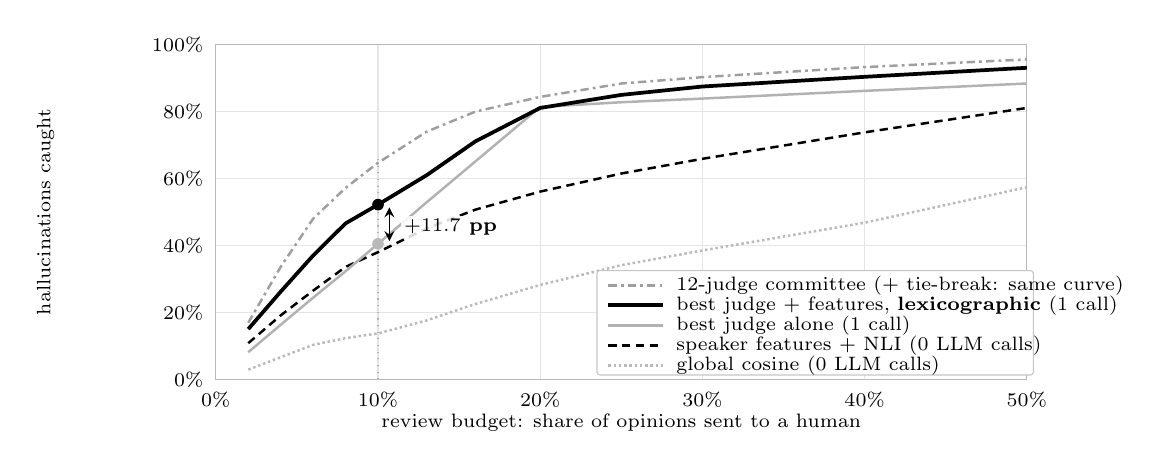
\begin{tikzpicture}[x=0.206cm, y=0.0425cm, font=\scriptsize,
                    c/.style={line width=0.9pt, line join=round},
                    comite/.style={c, gray!75, dash pattern=on 3pt off 1.5pt on 1pt off 1.5pt},
                    jlex/.style={c, line width=1.35pt},
                    juiz/.style={c, gray!60},
                    fam/.style={c, densely dashed},
                    cosg/.style={c, gray!55, densely dotted}]
  \draw[gray!20] (0,0) grid[xstep=10, ystep=20] (50,100);
  \draw[gray!55] (0,0) rectangle (50,100);
  \foreach \x in {0,10,20,30,40,50} \node[below=1pt] at (\x,0) {\x\%};
  \foreach \yy in {0,20,40,60,80,100} \node[left=1pt] at (0,\yy) {\yy\%};
  \node[below=9pt] at (25,0) {review budget: share of opinions sent to a human};
  \node[rotate=90] at (-10.5,50) {hallucinations caught};
  \draw[gray!60, dotted] (10,0) -- (10,66);
  \draw[cosg] plot coordinates {(2,2.9) (4,6.6) (6,10.3) (8,12.3) (10,13.7) (13,17.6) (16,22.5) (20,28.2) (25,34.1) (30,38.5) (40,46.8) (50,57.4)};
  \draw[fam] plot coordinates {(2,10.8) (4,19.1) (6,26.5) (8,33.6) (10,38.0) (13,45.1) (16,50.7) (20,56.1) (25,61.5) (30,65.9) (40,73.8) (50,81.1)};
  \draw[juiz] plot coordinates {(2,8.1) (4,16.3) (6,24.4) (8,32.3) (10,40.5) (13,52.9) (16,65.1) (20,81.4) (25,82.8) (30,83.9) (40,86.2) (50,88.4)};
  \draw[jlex] plot coordinates {(2,15.0) (4,26.2) (6,37.0) (8,46.6) (10,52.2) (13,61.0) (16,71.1) (20,81.1) (25,85.0) (30,87.5) (40,90.4) (50,93.1)};
  \draw[comite] plot coordinates {(2,16.9) (4,33.6) (6,48.0) (8,57.2) (10,64.7) (13,74.0) (16,80.0) (20,84.4) (25,88.4) (30,90.3) (40,93.3) (50,95.6)};
  \fill (10,52.2) circle (2.1pt); \fill[gray!55] (10,40.5) circle (2.1pt);
  \draw[<->, >=stealth, line width=0.6pt] (10.7,41.3) -- (10.7,51.4);
  \node[anchor=west, inner sep=1pt, fill=white, fill opacity=0.85,
        text opacity=1] at (11.4,45.5) {\textbf{$+11.7$ pp}};
  % legend
  \begin{scope}[shift={(24.2,2.5)}]
    \draw[fill=white, draw=gray!45, rounded corners=1pt] (-0.7,-1.2) rectangle (26.2,30);
    \draw[comite] (0,25.6) -- (3.4,25.6);
      \node[anchor=west, inner sep=1.5pt] at (3.9,25.6) {12-judge committee ($+$ tie-break: same curve)};
    \draw[jlex]   (0,19.6) -- (3.4,19.6);
      \node[anchor=west, inner sep=1.5pt] at (3.9,19.6) {best judge $+$ features, \textbf{lexicographic} (1 call)};
    \draw[juiz]   (0,13.6) -- (3.4,13.6);
      \node[anchor=west, inner sep=1.5pt] at (3.9,13.6) {best judge alone (1 call)};
    \draw[fam]    (0,7.6) -- (3.4,7.6);
      \node[anchor=west, inner sep=1.5pt] at (3.9,7.6) {speaker features + NLI (0 LLM calls)};
    \draw[cosg]   (0,1.6) -- (3.4,1.6);
      \node[anchor=west, inner sep=1.5pt] at (3.9,1.6) {global cosine (0 LLM calls)};
  \end{scope}
\end{tikzpicture}
\caption{Share of hallucinations found as a function of the review budget.
The curve of the best judge alone is a straight line up to $20\%$: a binary
verdict does not order the opinions within each of its two classes, so the
queue is in random order there. Ordering these ties with the
speaker-incidence features adds $11.7$ percentage points at a $10\%$ budget
with one judge call; with twelve judges the difference is not measurable.}
\label{fig:fila}
\end{figure}

At the inexpensive levels, the operational gain is large and agrees with the
theory. When one opinion in ten is reviewed, the global-cosine baseline finds
$13.7\%$ of the hallucinations, the speaker-incidence features $38.0\%$ without LLM-judge calls (with local NLI), and a single judge combined with them $52.2\%$, against
$40.5\%$ for the same judge alone. This single-judge gap follows from
Equation~\eqref{eq:captura} with $\tau = 26.1\%$: a binary judge ties most
pairs, so most of its queue is unordered.

With twelve judges, however, the gain in the queue is not measurable. We
hypothesised that the lexicographic queue would outperform the
committee's at every review budget. It does not: the differences are $-0.2$,
$+0.3$ and $+0.6$ percentage points at budgets of $5\%$, $10\%$ and $20\%$,
and every hearing-clustered interval includes zero. The location of the
committee's ties explains why. Three quarters of the tied pairs involve
opinions with zero or one vote (Figure~\ref{fig:comite}), and these opinions
occupy the last $69\%$ of the committee's queue: ordering them raises the
AUROC but does not change which opinions are reviewed under any budget below
$30\%$. Within such a budget only the vote level at the boundary is tied, and
even a perfect ordering of that level could change the recall by at most
$1.7$ to $4.7$ points. At twelve judges the result is therefore a ranking
improvement, not a workload improvement. For the selected single judge it improves both metrics, because the
best judge's single tied class of flagged opinions spans the first $20\%$ of
its queue.

\subsection{Controls}
\label{sec:res-controles}

Ordering the ties at random has the same expected AUROC as not ordering
them, but a non-negligible variance (over $200$ draws: mean $0.9259$, standard
deviation $0.0020$, maximum $0.9308$); against this distribution the
lexicographic result of $0.9300$ has $p = 0.015$. A deliberately weak
secondary detector, the global cosine ($\alpha = 0.5409$), gives a
non-significant $+0.0021$ $[-0.0017,+0.0057]$, as its low $\alpha$ predicts.
The committee must come first: reversing the order would lose the guarantee of
Proposition~\ref{thm:lex}(i).

% =============================================================================
\section{Measured Cost}
\label{sec:custo}

``Low cost'' needs evidence. We measured CPU time on a machine with $4$ vCPUs
and no GPU, and the tokens a judge reads (XLM-R tokenizer as a proxy;
Table~\ref{tab:custo}). We did not measure monetary cost, since provider
prices change.

\begin{table}[!ht]
  \centering
  \caption{Measured cost. The last two rows are per judge call; the judges'
  fixed prompt text is not included.}
  \label{tab:custo}
  \small
  \begin{tabular}{@{}lr@{}}
    \toprule
    \textbf{Component} & \textbf{Cost} \\
    \midrule
    speaker parsing, name matching and incidence features & 0.17 ms / opinion \\
    embedding the transcript (once per hearing; 982 sentences on average) & 38.9 s / hearing \\
    \quad amortised over the 20.6 opinions of a hearing & $\approx$1.9 s / opinion \\
    NLI, ten sentence pairs & $\approx$3.2 s / opinion \\
    \midrule
    tokens read by one judge (4 chunks $+$ opinion) & 600 (median), 875 (p95) \\
    tokens of a whole transcript, for contrast (mean, 40 hearings) & 27\,283 \\
    \bottomrule
  \end{tabular}
\end{table}

The cosine features cost about $1.9$ s of CPU per opinion, dominated by
embedding the transcript (paid once per hearing); the speaker-incidence
computation itself takes under a millisecond. The measured components of the full secondary detector, including ten NLI
pairs, total about $5.1$ s per opinion. These component benchmarks exclude
opinion embedding and retrieval/index overhead; they are not end-to-end latency. Neither makes an LLM call, whereas each judge call reads about
$600$ tokens: twelve judges read about $7{,}200$ tokens per opinion and the
eight judges of our non-inferiority result about $4{,}800$.

% =============================================================================
\section{Ethics, Data Use and Limits of Use}
\label{sec:etica}

\paragraph{Data.} We use only PublicHearingBR, built from official public
transcripts of the Brazilian Chamber of Deputies \citep{camara}, under the terms
of the challenge, of the C\^amara dos Deputados and of Hugging Face. No other
personal data is collected; names are pseudonymised in the figures and text,
and no per-person score is reported.

\paragraph{Limits of use.} The detector flags \emph{opinions} for human review;
it does not rank or profile individuals, and a flag is not evidence that a person
did not express a view, since the labels are an upper bound on hallucination.
An opinion should not be attributed to, or withdrawn from, a named person on
the detector's output alone.

% =============================================================================
\section{Threats to Validity}
\label{sec:ameacas}

\paragraph{Negative results.}\label{sec:negativos} We report findings that contradicted our hypotheses. Conditioned entailment does not
outperform conditioned cosine similarity (Section~\ref{sec:res-orador}); at
twelve judges the combination does not improve the review queue
(Section~\ref{sec:res-fila}); opinions whose supporting sentences contradict
one another are not more often unsupported (AUROC $0.43$ to $0.46$); and
fitting the secondary detector within each committee class lowers $\alpha$, as
do the five other attempts of Section~\ref{sec:res-orcamento}.

\paragraph{Labels.} We retain the released four-chunk NLI labels
\citep{publichearingbr}; they may overestimate full-transcript hallucination.
The 206 hearings form one corpus, so transfer to other domains or
summarisation systems remains to be evaluated. The audit of Section~\ref{sec:auditoria}
characterises the positives but does not replace the labels.

\paragraph{Binary judges.} The maximum gain $\tau/2$ would shrink if the judges produced calibrated probabilities; our combination result is conditional on binary votes.

\paragraph{Speaker recovery.} Speakers are matched by name for $85.7\%$ of
the opinions, and matching errors are not necessarily conservative: excluding
hearings with sign-language interpretation ($1.1\%$ of the opinions) lowers
the main signal from $0.7455$ to $0.7314$. All entailment probabilities come
from a single multilingual NLI model.

\paragraph{Scope of the claims.} The gain over the full committee is small
($+0.0040$, clustered CI lower bound $+0.0005$) and rests on its consistency:
it holds in all twenty fold partitions and for all twelve individual judges
(the full-committee comparison has $p=0.015$ against random tie-breaking); the advantage over stacking
($+0.0038$, lower bound $+0.0001$) is of the same size, and stacking is itself unstable across fold partitions. The primary comparisons are the three of
Section~\ref{sec:res-principal}; the per-judge results, the decomposition of
Section~\ref{sec:res-orcamento} and the audit are exploratory.

% =============================================================================
\section{Conclusion}
\label{sec:conclusao}

Pooled verification scores cannot tell whether an opinion was expressed by
the person to whom it is attributed. On PublicHearingBR, conditioning on the
attributed speaker's turns raises the AUROC of an inexpensive detector from
$0.57$ to $0.76$ without LLM-judge calls. Adding such a detector to a committee of LLM judges,
however, requires care: fitting a single model on both can overturn the committee's strict ordering, and on this
dataset it falls below the committee in 19 of 20 fold partitions. In contrast, ranking by
the committee and using the inexpensive detector only to order its ties never
reverses a strict committee ordering, and its gain equals the tie fraction times the
detector's advantage over chance on the tied pairs. Both quantities can be
estimated on a small labelled sample, allowing average benefit to be estimated before
deployment, as we verified on held-out hearings. The tested alternatives did not robustly close the remaining gap, and
the features provide little aggregate signal on pairs the committee orders incorrectly.

\paragraph{Practical implications.} The main consequence is a reduction in
the number of LLM calls needed for a given accuracy. One judge call combined
with the rule raises a typical judge from $0.81$ to $0.88$, recovering about
$60\%$ of the difference to the full committee with one twelfth of its LLM
calls; with the best judge, a reviewer who checks the $10\%$ most suspect
opinions finds $52.2\%$ of benchmark positives instead of $40.5\%$. Exploratory subset comparisons suggest that eight judges with the rule
can approach twelve-judge performance, potentially saving a third of calls. For a new corpus, one can measure the tie
fraction of the available judges on a labelled sample, estimate the
detector's AUROC on the tied pairs, and adopt the rule where the forecast gain
$\tau(\alpha-\tfrac12)$ justifies it. Negative findings delimit when these gains translate into a better review queue.

\medskip\noindent\textbf{Reproducibility.} All numbers in this paper are
produced by the scripts in the \texttt{code/} directory of the public
repository (\url{https://github.com/caua-sathler/IdeiasEmRede-TopoIA}). Analyses use fixed random seeds and precomputed tables; feature extraction
and CPU remeasurement have separate commands. A bilingual interactive
dashboard and a review-queue demonstration accompany the code. We thank Instituto Kunumi
for the \emph{Ideias em Rede} challenge and the authors of PublicHearingBR.

% =============================================================================
\bibliography{references}

\end{document}
